\section{Phương pháp}

\subsection{Hồi quy tuyến tính}

Hồi quy tuyến tính (Linear Regression) là một trong những phương pháp cơ bản và phổ biến nhất trong \textit{Data Mining} và \textit{Machine Learning}, được sử dụng để mô hình hóa mối quan hệ giữa một biến phụ thuộc và một hoặc nhiều biến độc lập. Mục tiêu của mô hình là tìm ra một hàm tuyến tính tốt nhất để dự đoán giá trị đầu ra dựa trên dữ liệu đầu vào.

Giả định cốt lõi của hồi quy tuyến tính là tồn tại mối quan hệ tuyến tính giữa các biến, tức là đầu ra có thể được biểu diễn dưới dạng tổ hợp tuyến tính của các biến đầu vào.

\subsubsection*{Nguyên lý hoạt động:}

\begin{itemize}
    \item \textbf{Hồi quy tuyến tính đơn (một biến đầu vào):}
    \[
        y = wx + b
    \]
    Trong đó:
    \begin{itemize}
        \item $y$: biến phụ thuộc (giá trị cần dự đoán)
        \item $x$: biến độc lập
        \item $w$: hệ số hồi quy (trọng số)
        \item $b$: hệ số chệch (bias/intercept)
    \end{itemize}
    
    \item \textbf{Hồi quy tuyến tính đa biến:}
    \[
        y = w_1x_1 + w_2x_2 + \cdots + w_nx_n + b = \mathbf{w}^T \mathbf{x} + b
    \]
    Với:
    \[
        \mathbf{x} = [x_1, x_2, \ldots, x_n]^T,\quad 
        \mathbf{w} = [w_1, w_2, \ldots, w_n]^T
    \]
\end{itemize}

Để đánh giá chất lượng mô hình, hàm mất mát phổ biến được sử dụng là \textbf{Mean Squared Error (MSE)}:

\[
    \text{MSE} = \frac{1}{m} \sum_{i=1}^{m} \left( y^{(i)} - \hat{y}^{(i)} \right)^2
\]

Trong đó:
\begin{itemize}
    \item $m$: số lượng mẫu
    \item $y^{(i)}$: giá trị thực tế
    \item $\hat{y}^{(i)}$: giá trị dự đoán
\end{itemize}

Mục tiêu của quá trình huấn luyện là tìm bộ tham số $\mathbf{w}, b$ sao cho MSE được tối thiểu hóa. Điều này thường được thực hiện thông qua các phương pháp tối ưu như \textit{Gradient Descent} hoặc nghiệm giải tích (\textit{Normal Equation}).

\subsubsection*{Ưu điểm và hạn chế:}

\begin{itemize}
    \item \textbf{Ưu điểm:}
    \begin{itemize}
        \item Đơn giản, dễ triển khai và huấn luyện nhanh
        \item Dễ diễn giải, cho phép hiểu rõ ảnh hưởng của từng đặc trưng
        \item Hoạt động tốt với dữ liệu có quan hệ tuyến tính
    \end{itemize}
    
    \item \textbf{Hạn chế:}
    \begin{itemize}
        \item Không mô hình hóa được quan hệ phi tuyến
        \item Nhạy cảm với outliers
        \item Có thể bị underfitting nếu dữ liệu phức tạp
    \end{itemize}
\end{itemize}

Trong bài toán dự đoán giá nhà, hồi quy tuyến tính là một mô hình cơ sở (\textit{baseline}) hiệu quả, giúp mô tả mối quan hệ giữa các đặc trưng như diện tích, số phòng, vị trí và giá trị bất động sản. Mặc dù đơn giản, mô hình vẫn cung cấp khả năng dự đoán tốt và đặc biệt hữu ích trong việc phân tích mức độ ảnh hưởng của từng yếu tố.

\subsection{Random Forest}

Random Forest là một phương pháp học máy thuộc nhóm \textit{Ensemble Learning}, được đề xuất nhằm cải thiện độ chính xác và khả năng tổng quát hóa của mô hình bằng cách kết hợp nhiều cây quyết định (\textit{Decision Trees}). Phương pháp này có thể áp dụng cho cả bài toán phân loại và hồi quy.

Trong bài toán hồi quy (Random Forest Regression), mô hình dự đoán giá trị liên tục bằng cách lấy trung bình kết quả từ nhiều cây hồi quy.

\subsubsection*{Nguyên lý hoạt động:}

Giả sử có $T$ cây hồi quy \( f_1(x), f_2(x), \ldots, f_T(x) \). Mỗi cây được huấn luyện độc lập trên một tập dữ liệu con được tạo ra bằng phương pháp \textbf{Bootstrap Sampling} từ tập dữ liệu gốc $D$:

\[
D_t \sim \text{Bootstrap}(D), \quad t = 1, 2, \ldots, T
\]

Ngoài ra, tại mỗi nút của cây, chỉ một tập con ngẫu nhiên các đặc trưng \( \mathcal{F}_t \subseteq \mathcal{F} \) được sử dụng để tìm điểm chia tối ưu. Điều này giúp tăng tính đa dạng giữa các cây và giảm tương quan giữa chúng.

Việc phân chia dữ liệu tại mỗi nút dựa trên tiêu chí giảm thiểu sai số, thường sử dụng \textbf{Sum of Squared Errors (SSE)}:

\[
\text{SSE} = \sum_{i \in S} \left( y^{(i)} - \bar{y}_S \right)^2
\]

Trong đó:
\[
\bar{y}_S = \frac{1}{|S|} \sum_{i \in S} y^{(i)}
\]

Cây sẽ tiếp tục phát triển cho đến khi đạt các điều kiện dừng như:
\begin{itemize}
    \item Độ sâu tối đa
    \item Số mẫu tối thiểu tại một nút
    \item Mức giảm sai số không còn đáng kể
\end{itemize}

Sau khi huấn luyện, dự đoán cuối cùng của mô hình được tính bằng trung bình các dự đoán từ tất cả các cây:

\[
\hat{y} = \frac{1}{T} \sum_{t=1}^{T} f_t(x)
\]

\begin{itemize}
    \item $T$: số lượng cây
    \item $f_t(x)$: dự đoán của cây thứ $t$
    \item $\hat{y}$: giá trị dự đoán cuối cùng
\end{itemize}

\subsubsection*{Ưu điểm và hạn chế:}

\begin{itemize}
    \item \textbf{Ưu điểm:}
    \begin{itemize}
        \item Mô hình hóa tốt các quan hệ phi tuyến phức tạp
        \item Giảm overfitting nhờ cơ chế ensemble
        \item Ít nhạy cảm với nhiễu và outliers
        \item Tự động đánh giá mức độ quan trọng của đặc trưng
    \end{itemize}
    
    \item \textbf{Hạn chế:}
    \begin{itemize}
        \item Chi phí tính toán cao hơn hồi quy tuyến tính
        \item Khó diễn giải hơn (black-box hơn)
        \item Mô hình lớn, tốn bộ nhớ
    \end{itemize}
\end{itemize}

Trong bài toán dự đoán giá nhà, Random Forest cho phép mô hình hóa các mối quan hệ phi tuyến giữa các yếu tố như diện tích, vị trí địa lý, tiện ích xung quanh và giá trị bất động sản. Nhờ khả năng tổng hợp nhiều cây quyết định, mô hình mang lại độ chính xác cao và khả năng tổng quát hóa tốt hơn so với các phương pháp tuyến tính.


\subsection{XGBoost}
XGBoost (Extreme Gradient Boosting) là một thuật toán học máy mạnh mẽ thuộc nhóm ensemble learning, cụ thể là phương pháp boosting. Nó được thiết kế để tối ưu hiệu năng và tốc độ khi huấn luyện mô hình cây quyết định.
\subsubsection*{Nguyên lý hoạt động:}
XGBoost xây dựng mô hình bằng cách kết hợp nhiều cây quyết định theo từng vòng lặp. Mỗi cây mới được huấn luyện nhằm sửa lỗi của cây trước đó, giúp mô hình học tốt hơn theo thời gian.

\subsubsection*{1. Hàm mục tiêu}

Ở vòng boosting thứ \( t \), mô hình XGBoost tối ưu hàm mục tiêu sau:
\[
\mathcal{L}^{(t)} = \sum_{i=1}^{n} l(y_i, \hat{y}_i^{(t-1)} + f_t(x_i)) + \Omega(f_t)
\]

Trong đó:
\begin{itemize}
	\item \( l \): hàm mất mát (thường dùng MSE: \( l(y, \hat{y}) = (y - \hat{y})^2 \))
	\item \(\hat{y_i}^{(t-1)}\): dự đoán của mô hình tại bước t - 1
	\item \(f_t\): cây quyết định mới tại bước t
	\item \( \Omega(f_t) \): thành phần regularization giúp chống overfitting
\end{itemize}

\[\Omega(f)f_t  = \gamma T + \frac{1}{2} \lambda \sum_{j=1}^{T} w_j^2 \]

Trong đó:
\begin{itemize}
	\item \(T\): số lá của cây
	\item \(w_j\): trọng số lá thứ \(j\)
	\item \(\gamma, \lambda\): hệ số điều chỉnh độ phức tạp mô hình
\end{itemize}
\subsubsection*{2. Xấp xỉ Taylor bậc hai}

XGBoost sử dụng xấp xỉ Taylor bậc hai để làm trơn hàm mất mát:

\[
\mathcal{L}^{(t)} \approx \sum_{i=1}^{n} \left[ g_i f_t(x_i) + \frac{1}{2} h_i f_t^2(x_i) \right] + \Omega(f_t)
\]

Trong đó:
- \( g_i = \frac{\partial l(y_i, \hat{y}_i^{(t-1)})}{\partial \hat{y}_i^{(t-1)}} \) (đạo hàm bậc 1)
- \( h_i = \frac{\partial^2 l(y_i, \hat{y}_i^{(t-1)})}{\partial (\hat{y}_i^{(t-1)})^2} \) (đạo hàm bậc 2)

\subsubsection*{3. Tính giá trị tối ưu tại mỗi lá}

Với mỗi lá \( j \), tập mẫu thuộc lá là \( I_j \). Tổng gradient và hessian tại lá:

\[
G_j = \sum_{i \in I_j} g_i, \quad H_j = \sum_{i \in I_j} h_i
\]

Giá trị đầu ra tối ưu tại lá:

\[
w_j^* = -\frac{G_j}{H_j + \lambda}
\]

Giá trị hàm mục tiêu tại điểm cực tiểu:

\[
\mathcal{L}^{(t)} = -\frac{1}{2} \sum_{j=1}^{T} \frac{G_j^2}{H_j + \lambda} + \gamma T
\]

\subsubsection*{Quá trình huấn luyện:}
Quá trình huấn luyện XGBoost bao gồm các bước chính sau:

\begin{itemize}
	\item[1. ] \textbf{Khởi tạo mô hình:} Dự đoán ban đầu là giá trị trung bình (cho hồi quy) hoặc xác suất (cho phân loại).
	\item[2.] \textbf{Tính toán gradient và hessian:} Các gradient (\( g_i \)) và hessian (\( h_i \)) được tính cho mỗi mẫu dựa trên hàm mất mát.
	\item[3.] \textbf{Xây dựng cây quyết định:} Mỗi cây mới được xây dựng để tối ưu hóa hàm mất mát với việc sử dụng gradient và hessian.
	\item[4.] \textbf{Cập nhật dự đoán:} Dự đoán của mô hình được cập nhật bằng cách cộng thêm giá trị từ cây mới.
	\item[5.] \textbf{Regularization:} Thành phần regularization giúp kiểm soát độ phức tạp của mô hình và ngăn ngừa overfitting.
	\item[6.] \textbf{Lặp lại quá trình:} Các bước trên được lặp lại cho đến khi đạt số vòng lặp tối đa hoặc không còn cải thiện đáng kể.
\end{itemize}

XGBoost là một lựa chọn mạnh mẽ cho bài toán hồi quy dự đoán giá nhà nhờ vào khả năng xử lý các mối quan hệ phi tuyến tính phức tạp trong dữ liệu. Mô hình này sử dụng kỹ thuật boosting, giúp tăng cường độ chính xác qua từng vòng lặp bằng cách học từ các sai sót của các cây quyết định trước đó. Điều này giúp XGBoost cải thiện hiệu suất so với mô hình hồi quy tuyến tính, vốn chỉ phù hợp với mối quan hệ tuyến tính giữa các đặc trưng và giá trị dự đoán.

Khác biệt với Random Forest, XGBoost không chỉ tạo ra nhiều cây quyết định độc lập mà còn tập trung vào việc tối ưu hóa mỗi cây dựa trên gradient của hàm mất mát, giúp giảm sai số một cách hiệu quả. Mặc dù Random Forest có thể xử lý các mối quan hệ phi tuyến tính, nhưng XGBoost thường cho kết quả tốt hơn nhờ vào khả năng tối ưu hóa liên tục và điều chỉnh chính xác hơn qua mỗi vòng huấn luyện.

\subsection{GridSearchCV} 
GridSearchCV là một phương pháp được sử dụng để tìm kiếm và tối ưu các siêu tham số (hyperparameters) của một mô hình học máy, nhằm cải thiện độ chính xác và hiệu suất của mô hình. Nó thực hiện thử tất cả các tổ hợp các giá trị siêu tham số có thể có từ một "lưới" các giá trị đã được chỉ định trước.

\subsubsection*{Nguyên lý hoạt động:}
GridSearchCV tìm kiếm trong không gian siêu tham số bằng cách thử nghiệm với mọi giá trị của các tham số đã cho, sử dụng phương pháp k-fold cross-validation để đánh giá hiệu suất của mỗi kết hợp tham số. Mục tiêu là tìm ra bộ tham số có thể tối ưu hóa độ chính xác của mô hình.

Quá trình này có thể được mô tả như sau:
\[
\text{Best Parameters} = \arg \max_{\theta} \left( \frac{1}{k} \sum_{i=1}^{k} \text{score}(X_{train}^{(i)}, y_{train}^{(i)}, \theta) \right)
\]
Trong đó:
\begin{itemize}
	\item \( \theta \) là bộ tham số của mô hình.
	\item \( X_{train}^{(i)} \) và \( y_{train}^{(i)} \) là dữ liệu huấn luyện tại lần gập thứ \(i\) trong quá trình k-fold cross-validation.
	\item \(\text{score}(X, y, \theta)\) là độ chính xác của mô hình với tham số \(\theta\) trên bộ dữ liệu \(X\) và \(y\).
\end{itemize}
\subsubsection*{Tối ưu siêu tham số với GridSearchCV}
Trong bài toán này, nhóm sẽ kết hợp giữa phương pháp bagging và boosting cây quyết định, cụ thể là các mô hình Random Forest và XGBoost, với kỹ thuật GridSearchCV để tối ưu hóa các tham số của mô hình. Phương pháp bagging (Bootstrap Aggregating) được áp dụng với Random Forest, trong khi đó boosting được sử dụng với XGBoost, nhằm tăng cường hiệu quả dự đoán và giảm thiểu lỗi.

Cả hai mô hình Random Forest và XGBoost đều có các siêu tham số quan trọng có thể điều chỉnh để tối ưu hóa hiệu suất. Với GridSearchCV, nhóm sẽ tìm kiếm và chọn lựa các giá trị siêu tham số tối ưu thông qua việc thử nghiệm tất cả các kết hợp có thể của các tham số trong không gian tìm kiếm. Quá trình này giúp mô hình đạt được hiệu quả dự đoán tốt nhất cho bài toán cụ thể.

GridSearchCV sẽ giúp tìm ra các tham số tối ưu của mô hình thông qua việc đánh giá hiệu suất mô hình trên một tập kiểm tra (cross-validation) với các tham số khác nhau, từ đó chọn ra bộ tham số tối ưu giúp mô hình hoạt động hiệu quả nhất. Các tham số sẽ bao gồm:
\begin{itemize}
	\item \textbf{Random Forest:} số lượng cây (\textit{n\_estimators}), độ sâu tối đa của cây (\textit{max\_depth}), số lượng mẫu tối thiểu để chia tách (\textit{min\_samples\_split}).
	\item \textbf{XGBoost:} số lượng cây (\textit{n\_estimators}), tốc độ học (\textit{learning\_rate}), độ sâu của cây (\textit{max\_depth}), tỷ lệ mẫu (\textit{subsample}).
\end{itemize}

Việc kết hợp giữa bagging, boosting và GridSearchCV giúp mô hình cải thiện khả năng dự đoán trong các bài toán phức tạp như dự báo giá nhà, từ đó giúp mô hình có khả năng học được các mối quan hệ phi tuyến tính và giảm thiểu overfitting.

\subsection{Mạng nơ-ron nhiều lớp}
Mạng nơ-ron nhân tạo (Artificial Neural Network - ANN) là một mô hình tính toán được lấy cảm hứng từ cấu trúc và chức năng của hệ thần kinh sinh học. Trong đó, mạng nơ-ron nhiều lớp (Multilayer Perceptron - MLP) là một dạng mạng nơ-ron phổ biến và quan trọng, có khả năng học các mối quan hệ phi tuyến giữa đầu vào và đầu ra thông qua nhiều tầng xử lý thông tin. Mạng nơ-ron nhiều lớp là một loại mạng nơ-ron truyền thẳng (feedforward neural network), trong đó các nơ-ron được tổ chức thành từng tầng, bao gồm: tầng đầu vào, một hoặc nhiều tầng ẩn, và tầng đầu ra. Mỗi tầng đều gồm nhiều nơ-ron, trong đó mỗi nơ-ron của một tầng bất kỳ đều được kết nối đầy đủ với tất cả các nơ-ron của tầng liền trước và tầng liền sau, tạo thành một mạng có kết nối dày đặc (fully connected).

\begin{figure}[H]
	\centering
	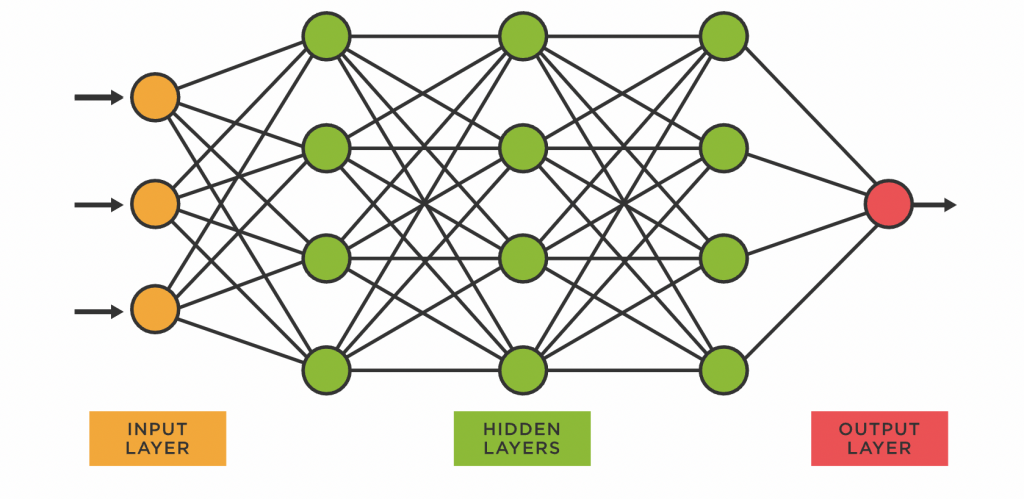
\includegraphics[width=1\linewidth]{chapters/PP/assets/R.png}
	\caption{Mạng nơ-ron nhân tạo nhiều lớp}
\end{figure}

\subsubsection*{Nguyên lý hoạt động:}

Quá trình xử lý dữ liệu trong MLP được chia thành hai giai đoạn chính: lan truyền tiến (forward propagation) và lan truyền ngược (backpropagation). Trong giai đoạn lan truyền tiến, dữ liệu đầu vào được truyền từ tầng đầu vào qua các tầng ẩn tới tầng đầu ra. Mỗi nơ-ron thực hiện phép biến đổi tuyến tính với trọng số và hệ số dịch như sau:

\[
z^{(l)} = W^{(l)} a^{(l-1)} + b^{(l)}, \quad a^{(l)} = \phi(z^{(l)})
\]

Trong đó:
\begin{itemize}
	\item $W^{(l)}$ là ma trận trọng số của tầng $l$
	\item $b^{(l)}$ là vector hệ số dịch (bias)
	\item $a^{(l-1)}$ là đầu ra của tầng trước
	\item $\phi$ là hàm kích hoạt phi tuyến
\end{itemize}

Sau khi đầu ra cuối cùng được tính toán, hàm mất mát (loss function) sẽ đo độ sai lệch giữa đầu ra dự đoán và nhãn thực tế. Hàm mất mát phổ biến trong bài toán phân loại là hàm cross-entropy, trong khi bài toán hồi quy thường dùng hàm MSE (Mean Squared Error).

Để cập nhật trọng số nhằm giảm sai số, thuật toán lan truyền ngược được sử dụng. Dựa trên đạo hàm của hàm mất mát đối với các trọng số, ta cập nhật từng trọng số theo hướng giảm gradient:

\[
W^{(l)} \leftarrow W^{(l)} - \eta \frac{\partial L}{\partial W^{(l)}}
\]

Trong đó $\eta$ là tốc độ học (learning rate), quyết định mức độ điều chỉnh sau mỗi lần cập nhật. Việc cập nhật có thể được thực hiện bằng nhiều thuật toán tối ưu khác nhau như Gradient Descent, Stochastic Gradient Descent (SGD), hay Adam — một phương pháp hiện đại và phổ biến vì khả năng hội tụ nhanh và ổn định.

\subsubsection*{Vai trò của hàm kích hoạt và khả năng biểu diễn phi tuyến}

Một điểm then chốt trong kiến trúc của MLP là việc sử dụng các hàm kích hoạt phi tuyến. Nếu toàn bộ mạng chỉ bao gồm các phép biến đổi tuyến tính, thì dù có nhiều tầng cũng không thể biểu diễn được hàm phi tuyến phức tạp. Hàm kích hoạt giúp mạng "bẻ cong" không gian đặc trưng, từ đó học được các mối quan hệ phức tạp trong dữ liệu.

Một số hàm kích hoạt phổ biến như:

\begin{itemize}
	\item \textbf{Sigmoid:} thích hợp cho đầu ra nhị phân nhưng dễ bị "vanishing gradient".
	\item \textbf{Tanh:} cải tiến so với sigmoid do có đầu ra đối xứng quanh 0, nhưng vẫn bị mất gradient ở biên.
	\item \textbf{ReLU:} đơn giản và hiệu quả, giúp giải quyết vấn đề mất gradient, tuy nhiên có thể bị "chết nơ-ron" nếu giá trị đầu vào âm liên tục.
	\item \textbf{Leaky ReLU:} một biến thể của ReLU có thể giải quyết vấn đề chết nơ-ron bằng cách cho phép gradient nhỏ hơn 0 ở phía âm.
\end{itemize}

Nhờ vào các hàm kích hoạt này, MLP có thể xấp xỉ bất kỳ hàm liên tục nào, theo định lý xấp xỉ phổ quát (Universal Approximation Theorem), nếu được cung cấp đủ nơ-ron và dữ liệu huấn luyện phù hợp.

Trong khi các phương pháp hồi quy tuyến tính hoặc cây quyết định có thể tốt với các mối quan hệ đơn giản hoặc có cấu trúc rõ ràng, MLP có thể học được các mối quan hệ không tuyến tính mà các phương pháp này không thể mô phỏng được. Điều này đặc biệt quan trọng trong dự báo giá nhà, vì giá trị bất động sản thường bị ảnh hưởng bởi nhiều yếu tố phức tạp, chẳng hạn như vị trí, kích thước, tình trạng tài chính của người mua, hoặc các yếu tố kinh tế vĩ mô mà không thể dễ dàng mô hình hóa bằng các phương pháp thông thường.

Với khả năng xấp xỉ các hàm phi tuyến, MLP có thể nắm bắt các mẫu dữ liệu phức tạp và linh hoạt hơn, đặc biệt khi dữ liệu huấn luyện có nhiều đặc trưng và mối quan hệ giữa chúng không phải là tuyến tính. Đột phá của MLP so với các phương pháp truyền thống là khả năng học từ dữ liệu mà không cần phải đưa ra giả định về mối quan hệ giữa các đặc trưng. MLP có thể tự động tìm ra các mối quan hệ phi tuyến, điều mà các mô hình hồi quy tuyến tính không thể thực hiện, từ đó nâng cao độ chính xác của dự báo giá nhà, đặc biệt trong các trường hợp có sự thay đổi hoặc biến động mạnh trong các yếu tố ảnh hưởng.
